%!TEX root = gorila_paper.tex
\section{Experiments}
\subsection{Experimental Set Up}
We evaluated Gorila by conducting experiments on 49 Atari 2600 games using the Arcade Learning Environment~\cite{bellemare-ale}.
Atari games provide a challenging and diverse set of reinforcement learning problems where an agent must learn to play the games directly from $210\times 160$ RGB video input with only the changes in the score provided as rewards.
We closely followed the experimental setup of DQN~\cite{mnih-dqn-2015} using the same preprocessing and network architecture.
We preprocessed the $210\times 160$ RGB images by downsampling them to $84\times 84$ and extracting the luminance channel.

The Q-network $Q(s,a;\theta)$ had 3 convolutional layers followed by a fully-connected hidden layer.
The $84\times 84\times 4$ input to the network is obtained by concatenating the images from four previous preprocessed frames.
The first convolutional layer had $32$ filters of size $4\times 8\times 8$ and stride $4$. The second convolutional layer had $64$ filters of size $32\times 4\times 4$ with stride $2$, while the third had $64$ filters with size $64\times 3\times 3$ and stride $1$. The next layer had $512$ fully-connected output units, which is followed by a linear fully-connected output layer with a single output unit for each valid action. 
Each hidden layer was followed by a rectifier nonlinearity.

We have used the same frame skipping step implemented in~\cite{mnih-dqn-2015} by repeating every action $a_t$ over the next $4$ frames. 

In all experiments, Gorila DQN used: $N_{param}=31$ and $N_{learn} = N_{act} =$ 100. We use the bundled mode. Replay memory size $D=$ 1 million frames and used $\epsilon$-greedy as the behaviour policy with $\epsilon$ annealed from 1 to 0.1 over the first one million global updates.
Each learner syncs the parameters $\theta^-$ of its target network after every 60K parameter updates performed in the parameter server.


\begin{figure*}[!ht]
	\vskip -0.1in
	\begin{center}
		\centerline{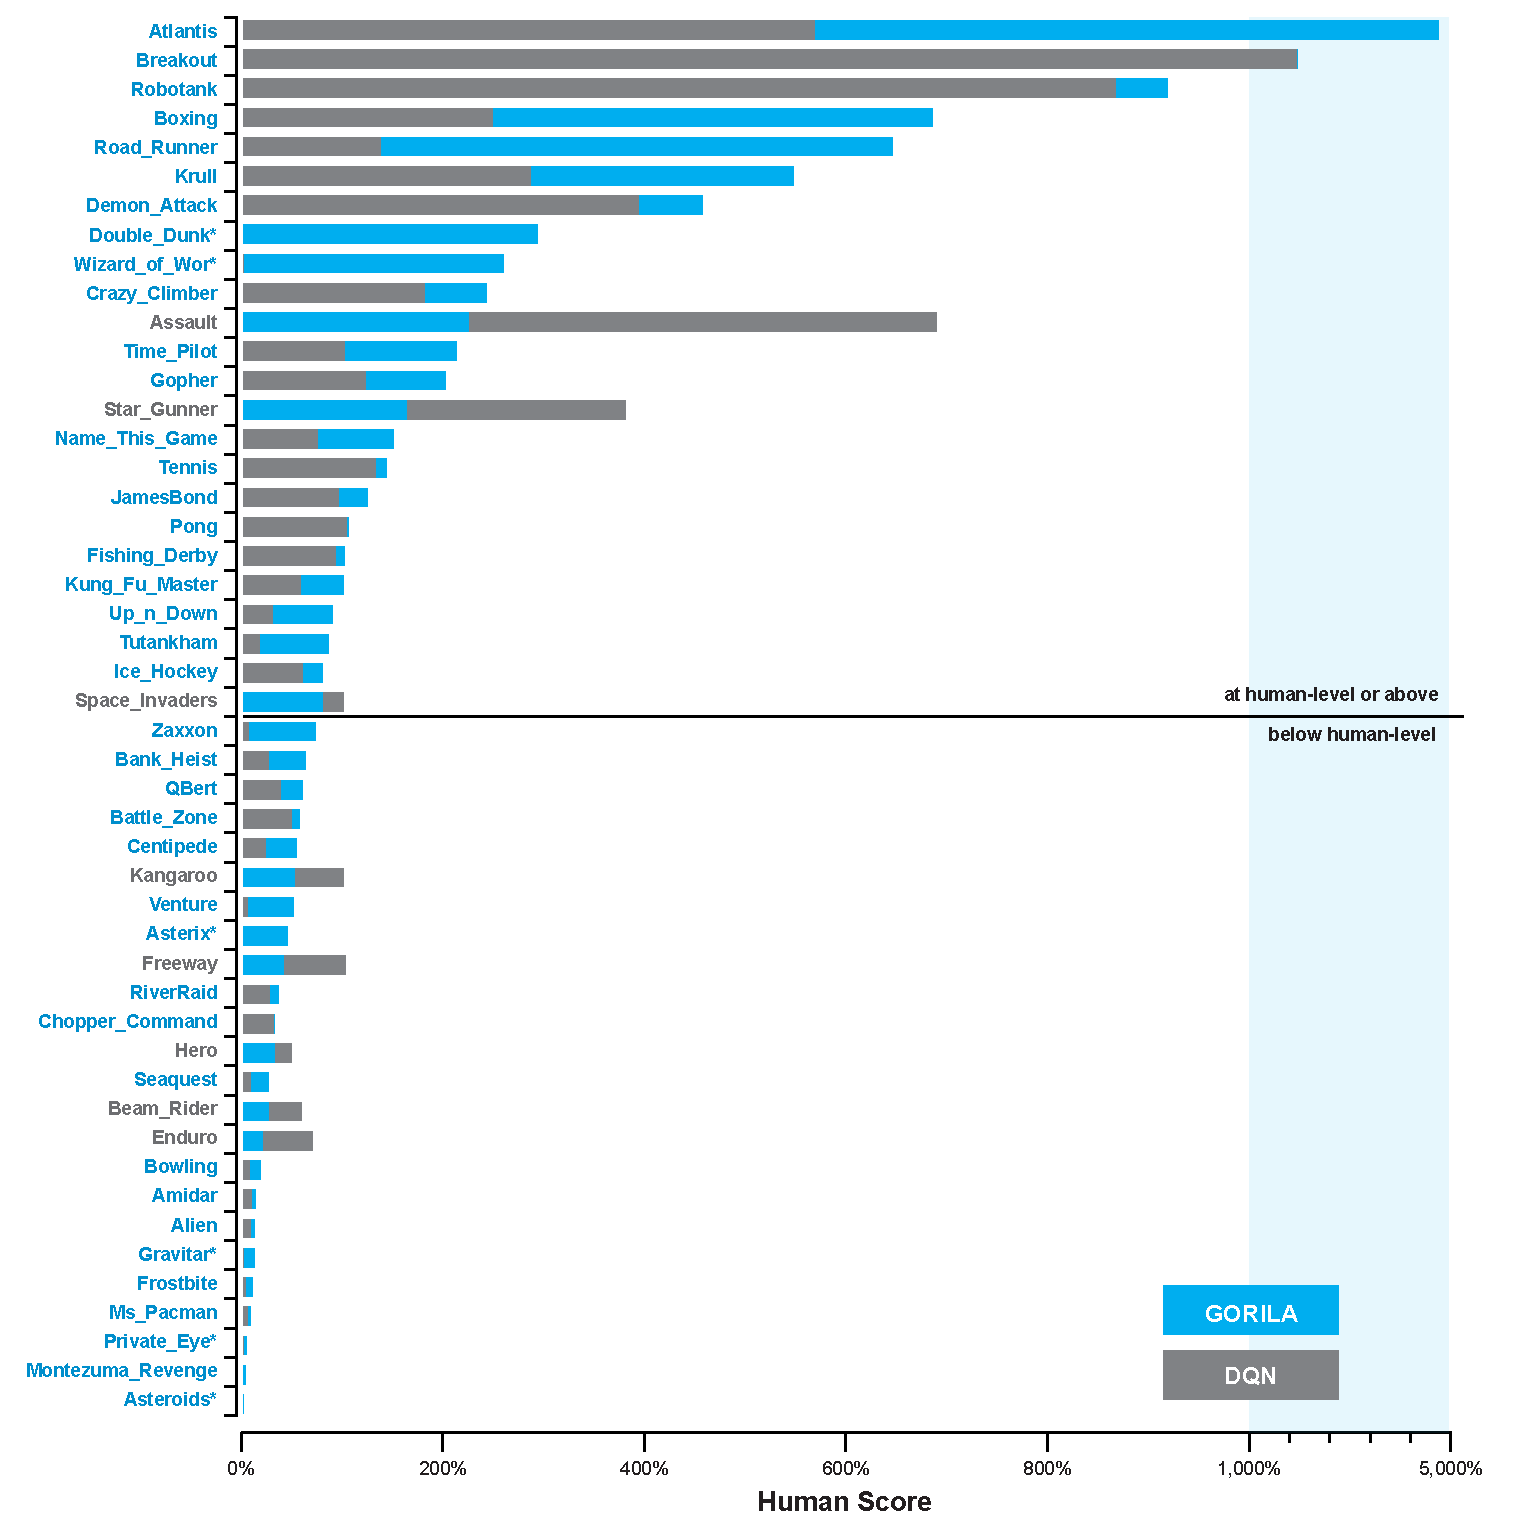
\includegraphics[width=0.95\textwidth]{GorilaHuman3}}
		\caption{Performance of the Gorila agent on 49 Atari games with human starts evaluation compared with DQN~\cite{mnih-dqn-2015} performance with scores normalized to expert human performance.  Font color indicates which method has the higher score. *Not showing DQN scores for Asterix, Asteroids, Double Dunk, Private Eye, Wizard Of Wor and Gravitar because the DQN human starts scores are less than the random agent baselines. Also not showing Video Pinball because the human expert scores are less than the random agent scores.}
		\label{fig:humanstarts}
	\end{center}
	\vskip -0.2in
\end{figure*}

\begin{figure*} [!ht]
	\vskip -0.1in
	\begin{center}
		\centerline{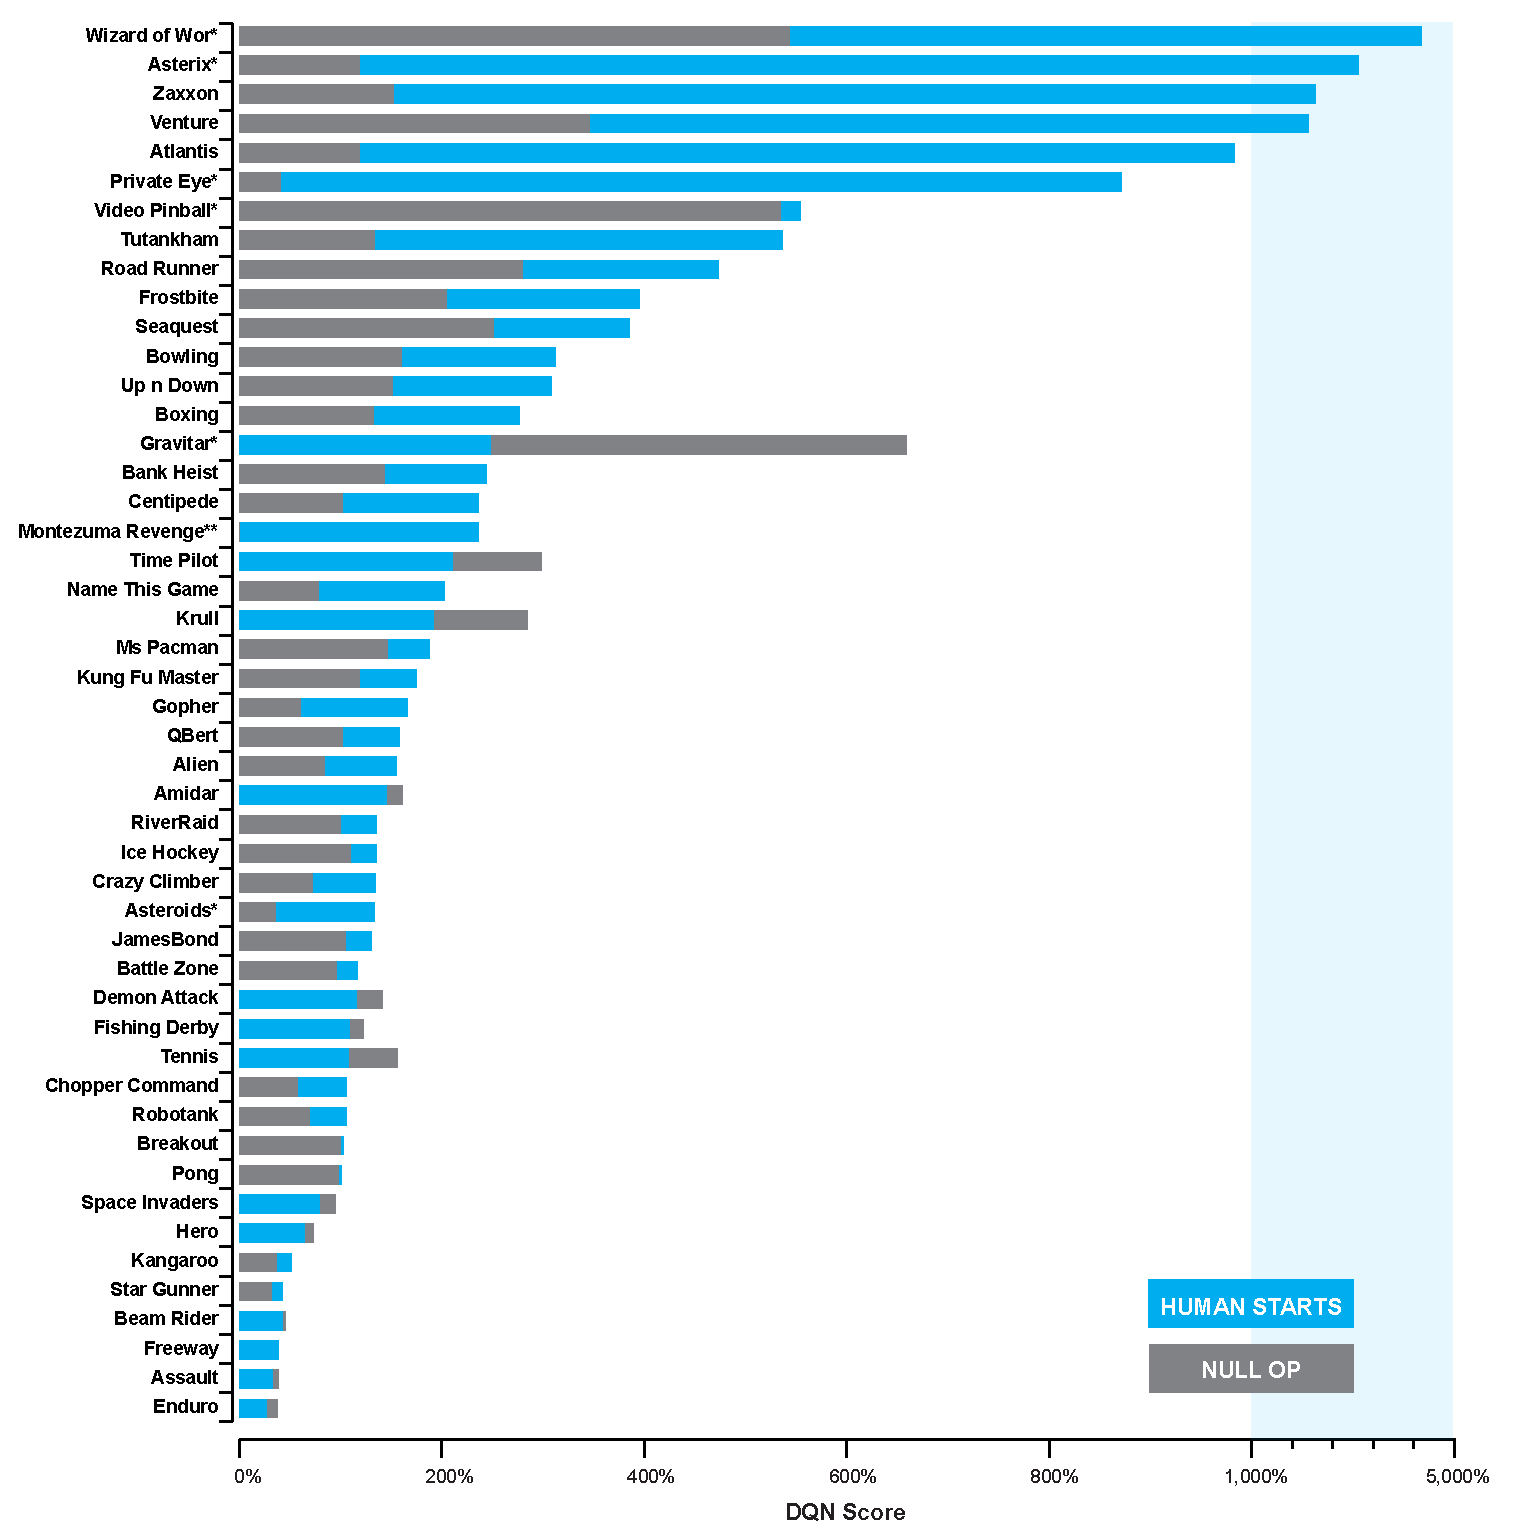
\includegraphics[width=0.95\textwidth]{GorilaMixture5}}
		\caption{Performance of the Gorila agent on 49 Atari games with human starts and null op evaluations normalized with respect to DQN human start and null op scores respectively. This figure shows the generalization improvements of Gorila compared to DQN. *Using a score of 0 for the human starts random agent score for Asterix, Asteroids, Double Dunk, Private Eye, Wizard Of Wor and Gravitar because the human starts DQN scores are less than the random agent scores. Not showing Double Dunk because both the DQN scores and the random agent scores are negative. **Not showing null op scores for Montezuma Revenge because both the human start scores and random agent scores are 0.
		}
		\label{fig:humanstarts1}
	\end{center}
	\vskip -0.2in
\end{figure*}

\subsection{Evaluation}

We used two types of evaluations.
The first follows the protocol established by DQN. Each trained agent was evaluated on 30 episodes of the game it was trained on.
A random  number of frames were skipped by repeatedly taking the null or do nothing action before giving control to the agent in order to ensure variation in the initial conditions.
The agents were allowed to play until the end of the game or up to 18000 frames (5 minutes), whichever came first, and the scores were averaged over all 30 episodes. We refer to this evaluation procedure as {\it null op starts}.

Testing how well an agent generalizes is especially important in the Atari domain because the emulator is completely deterministic.

Our second evaluation method, which we call {\it human starts}, aims to measure how well the agent generalizes to states it may not have trained on. To that end, we have introduced 100 random starting points that were sampled from a human professional's gameplay for each game.
To evaluate an agent, we ran it from each of the 100 starting points until the end of the game or until a total of 108000 frames (equivalent to 30 minutes) were played counting the frames the human played to reach the starting point.
The total score accumulated only by the agent (not considering any points won by the human player) were averaged to obtain the evaluation score.


In order to make it easier to compare results on 49 games with a greatly varying range of scores we present the results on a scale where 0 is the score obtained by a random agent and 100 is the score obtained by a professional human game player.
%~\footnote{We also included the raw scores obtained by all agents in the Appendix for reference.}.
The random agent selected actions uniformly at random at 10Hz and it was evaluated using the same starting states as the agents for both kinds of evaluations ({\it null op} starts and {\it human starts}).

We selected hyperparameter values by performing an informal search on the games of Breakout, Pong and Seaquest which were then fixed for all the games.
We have trained Gorila DQN 5 times on each game using the same fixed hyperparameter settings and random network initializations. Following DQN, we periodically evaluated each model during training and kept the best performing network parameters for the final evaluation. We average these final evaluations over the 5 runs, and compare the mean evaluations with DQN and human expert scores.

